%================================================================
%\chapter{Selection of Standard Probability Distributions}\label{sec:Appendix A}
\chapter{Additional Results}\label{sec:Appendix A}
%================================================================


\begin{figure}[H]
    \centering
    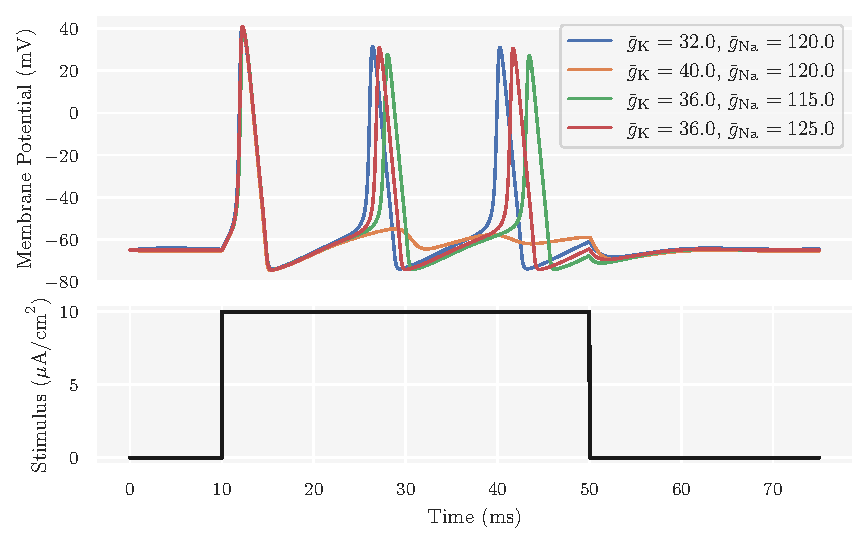
\includegraphics[scale=1.0]{hh_different_gs}
    \caption{Simulation of action potentials with the Hodgkin-Huxley simulator for different values of $\gbarK$ and $\gbarNa$ (stated in the legend). The rest of the parametrization is given by \autoref{tab:hh_model_parameters}.
    }
    %\label{fig:hh_different_gs}
\end{figure}


\begin{figure}[H]
    \centering
    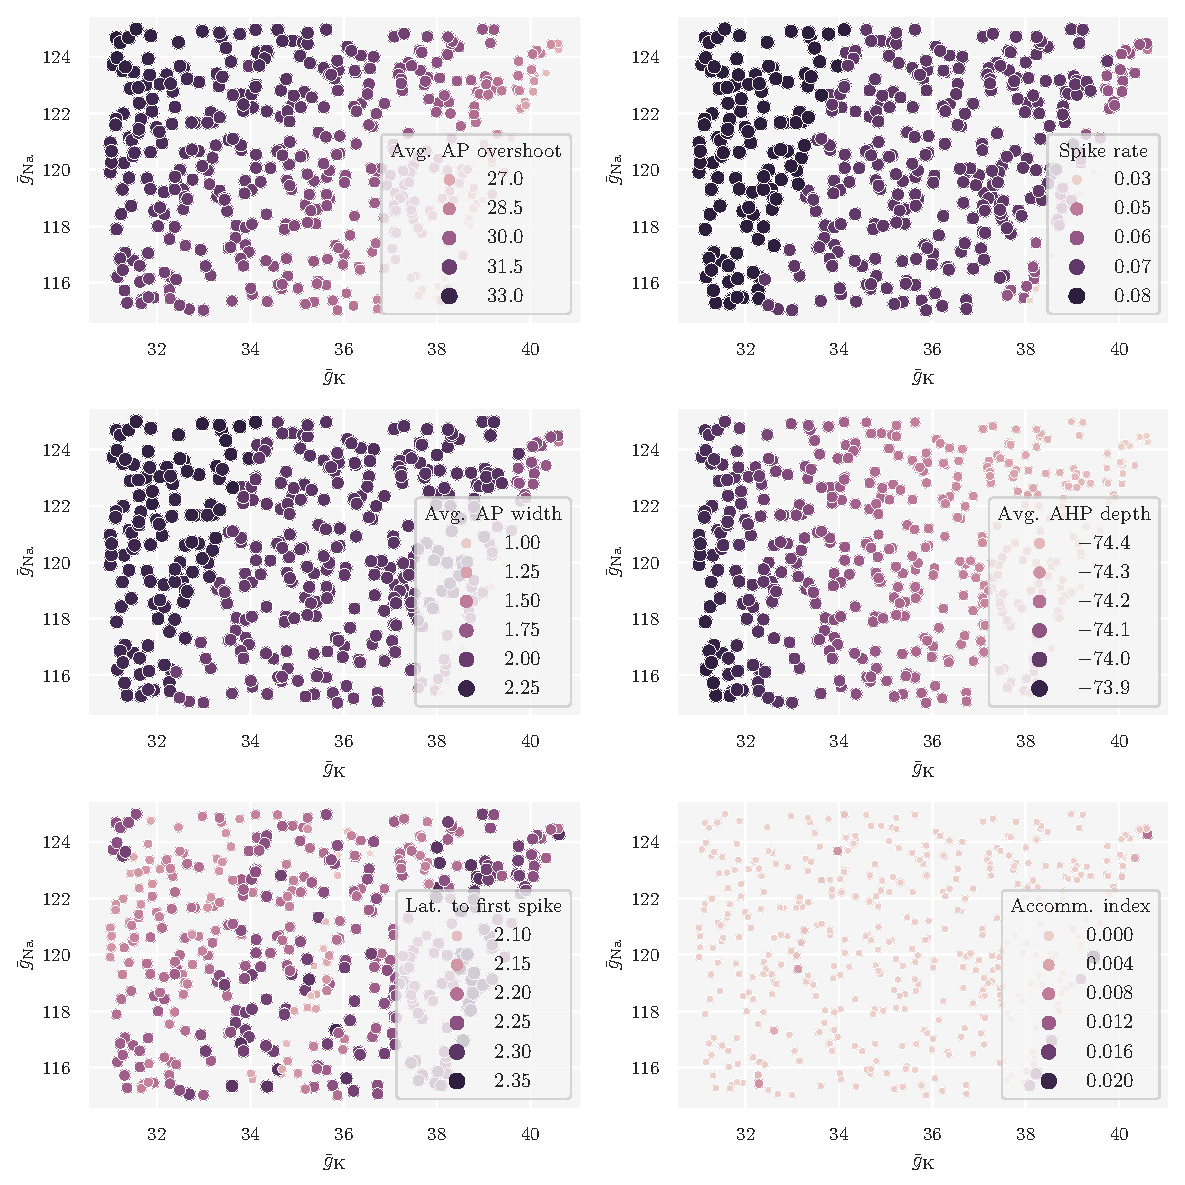
\includegraphics[scale=0.7]{hh_priorpred_sstats_uniform}
    \caption{Similar to \autoref{fig:hh_priorpred_sstats_normal}, only with summary statistics simulated under the joint noninformative prior distribution. Of the 2000 samples generated, 1703 were well-defined. Here a subset of 425 samples is shown.}
    %\label{fig:fig1}
\end{figure} 

% subfigure
\begin{figure}[H]
\centering
\subfloat[]{{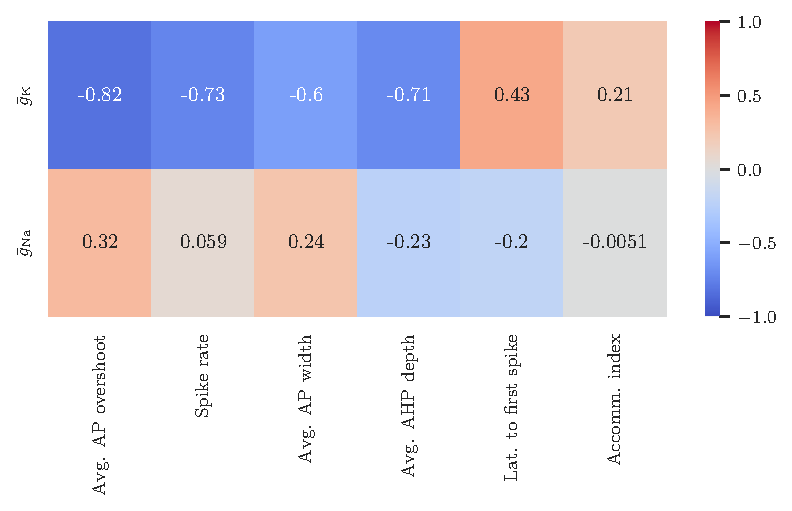
\includegraphics[scale=0.65]{hh_priorpred_corr_uniform}}}
\qquad
\subfloat[]{{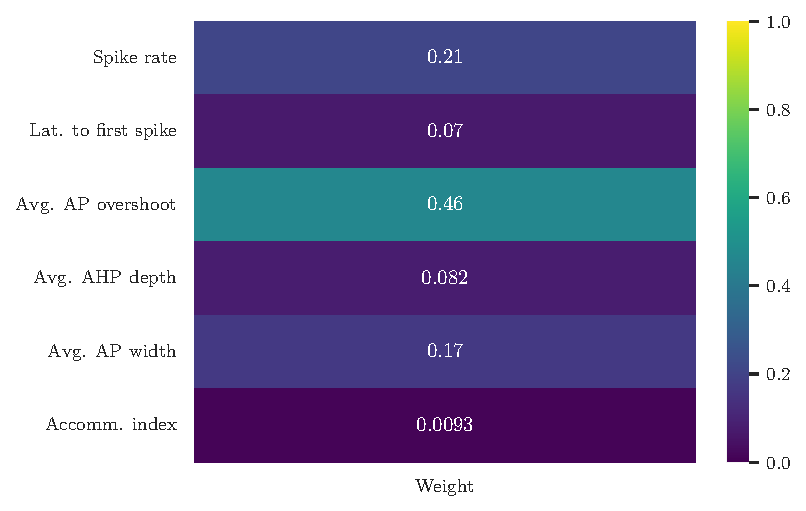
\includegraphics[scale=0.65]{hh_priorpred_weights_uniform}}}
\caption{Similar to \autoref{fig:hh_weights_normal}, but with samples from the joint noninformative prior distribution. \textbf{(a)} The pairwise Pearson's correlation coefficients. \textbf{(b)} Importance weights calculated from the correlation coefficients (summed to 1).
}
%\label{fig:hh_weights_uniform}
\end{figure}


 
%REJ-ABC hyperparam study 

%Run time

\begin{figure}[H]
    \centering
    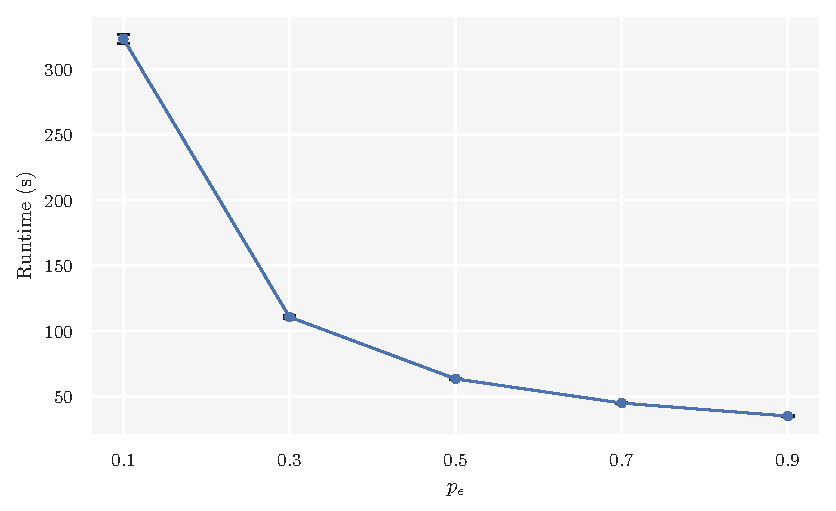
\includegraphics[scale=0.8]{comp_time_quantile}
    \caption{Illustration of computational run time for obtaining 1000 posterior samples with the HH simulator vs. tolerance quantile, i.e., the proportion of simulations that are accepted.}
    %\label{fig:fig1}
\end{figure}

%num of pilot study simulations 

\begin{figure}[H]
    \centering
    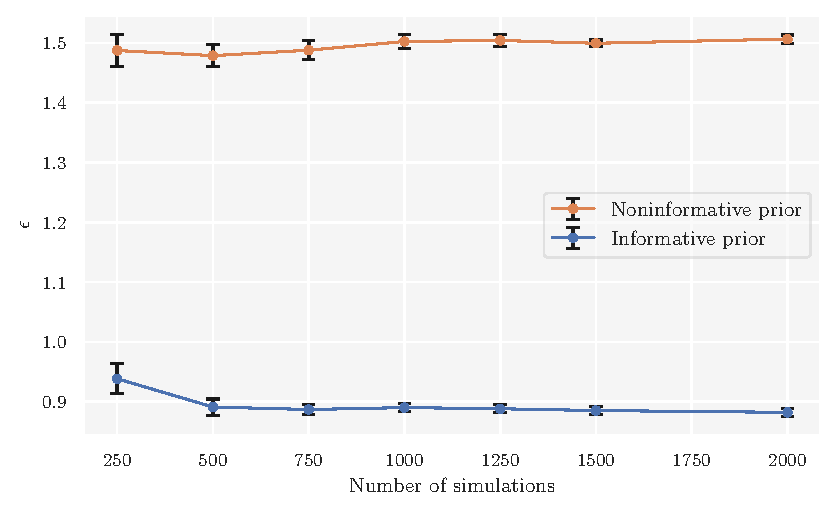
\includegraphics[scale=0.8]{pilot_eps_nsims}
    \caption{Estimated tolerance $\epsilon$ vs. the number of simulations in the pilot study. Here, both summary statistic scales and weights are set to 1 when calculating the distance, so the estimates might not be representative for all use cases.}
    %\label{fig:fig1}
\end{figure} 

%num of posterior draws

%\begin{figure}[H]
%    \centering
%    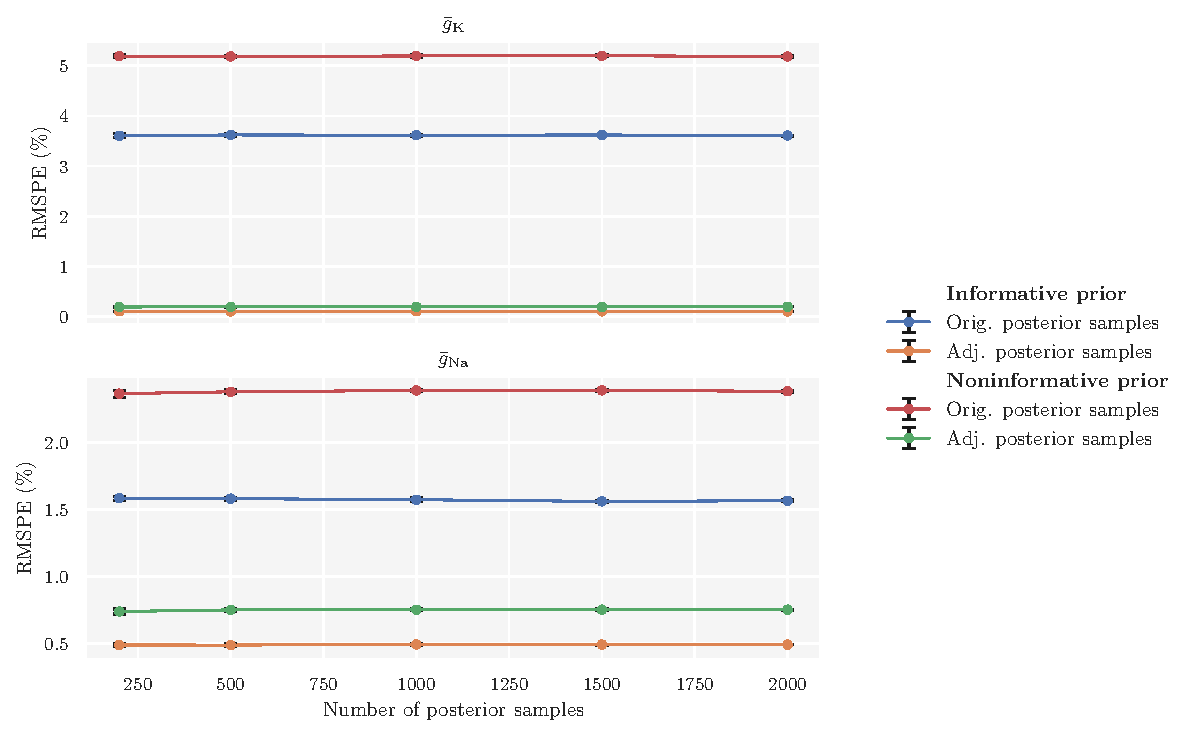
\includegraphics[scale=0.8]{RMSPE_vs_nsamples}
%    \caption{caption}
%    \label{fig:fig1}
%\end{figure} 


%Brunel joint posterior (original) (REMOVE?)

%\begin{figure}[H]
%    \centering
%    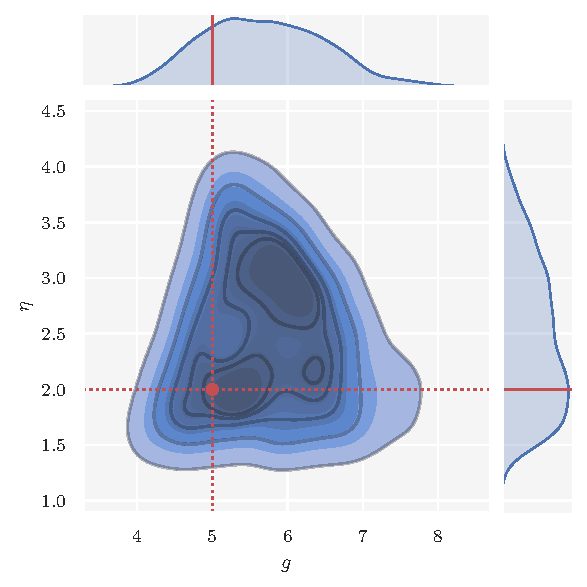
\includegraphics[scale=1.0]{brunel_joint_posterior_org}
%    \caption{caption}
%    \label{fig:fig1}
%\end{figure} 



